\documentclass[12pt,a4paper]{article}
\usepackage[UTF8]{ctex}     %先引入ctex
\usepackage[utf8]{inputenc} %再引入inputenc
\usepackage{graphicx}
\usepackage{geometry}
\usepackage{xcolor}
% \usepackage{lazylatex}
\usepackage{amsmath}
\usepackage{enumerate}
\usepackage{caption}
\usepackage{listings}
\captionsetup[lstlisting]{labelfont=bf,justification=justified}

\usepackage{tikz}
\usepackage{appendix}

\graphicspath{{img/}}
% 边距
\geometry{left=2.0cm,right=2.0cm,top=2.0cm,bottom=3.0cm}
% 大题
\newenvironment{problems}{\begin{list}{}{\renewcommand{\makelabel}[1]{\textbf{##1}\hfil}}}{\end{list}}
% 小题
\newenvironment{steps}{\begin{list}{}{\renewcommand{\makelabel}[1]{##1.\hfil}}}{\end{list}}
% 答
\providecommand{\ans}{\textbf{答}:~}
% 解
\providecommand{\sol}{\textbf{解}.~}

\usepackage[colorlinks,linkcolor=blue]{hyperref}
\usepackage{bookmark}
\providecommand{\code}[2]{\lstinputlisting[language=#2,caption=\href{run:#1}{\ttfamily #1}]{#1}}
\providecommand{\img}[1]{\includegraphics[width=0.88\textwidth]{#1}}

% listings
\definecolor{grey}{rgb}{0.8,0.8,0.8}
\definecolor{darkgreen}{rgb}{0,0.3,0}
\definecolor{darkblue}{rgb}{0,0,0.3}
\lstset{%
    % numbers=left, %行号
    % numberstyle=\tiny\color{grey},
    showstringspaces=false,
    showspaces=false,%
    tabsize=4,%
    frame=shadowbox,%
    basicstyle={\ttfamily\scriptsize},%
    keywordstyle=\color{blue!80!black}\bfseries,%
    identifierstyle=,%
    commentstyle=\color{green!50!blue}\itshape,%
    stringstyle=\color{green!50!black},%
    rulesepcolor=\color{gray!20!white},
    breaklines,
    columns=flexible,
    extendedchars=false,
    %mathescape=true,
}

\begin{document}
\title{\normalsize \underline{操作系统(D)}\\\LARGE 项目 3}
\author{Log Creative }
\date{\today}
\maketitle

\begin{problems}
    \item[一] \textbf{多线程排序程序}
    
    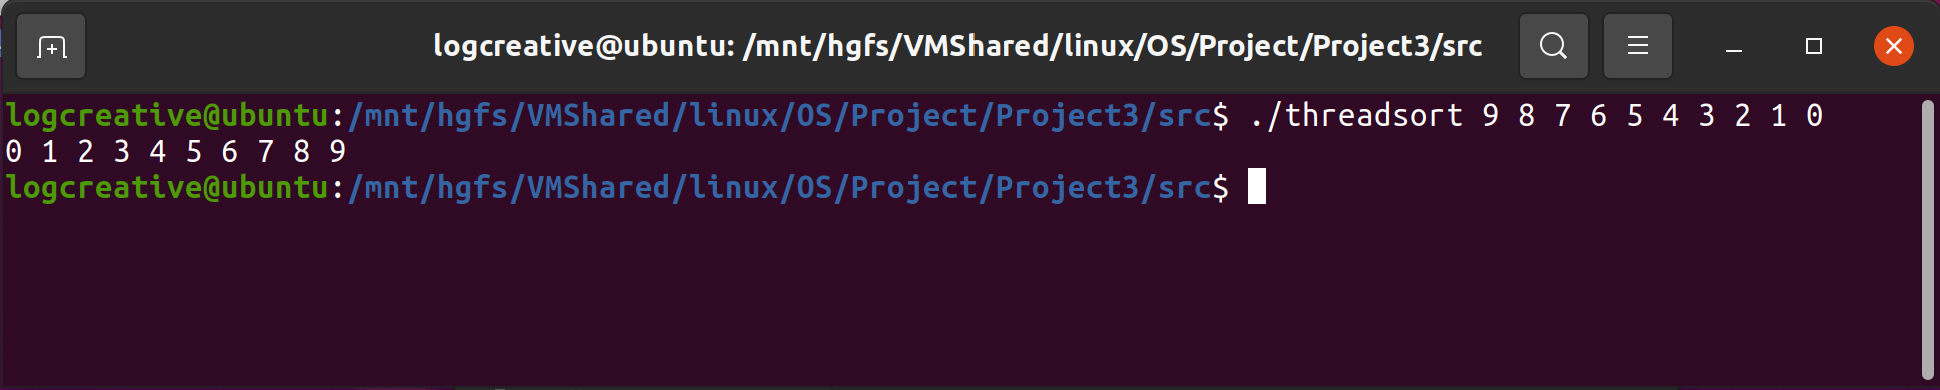
\includegraphics[width=0.9\textwidth]{threadsort.png}

    使用命令行的参数获取需要排序的数组,使用动态内存分配原数组和排序数组。原数组两边分别开一个线程用冒泡排序,最后归并两个数组到排序数组中。定义了一个结构体用于传递参数:
    \begin{lstlisting}[language=c]
typedef struct {
    int start;
    int end;
} sort_param;
    \end{lstlisting}

    \code{src/threadsort.c}{c}

    \item[二] \textbf{分离--联合排序程序} 
    
    使用 java 实现快速排序和归并排序的多线程版本。当需要排序的数组量小于阈值 \verb"THRESHOLD" 100 时,将会采用选择排序。派生了了 \verb"RecursiveAction" 类用于多线程运算。使用 \verb"Comparable" 用于任何可比较类型的比较。

    取消 \verb"main" 函数开始时的注释,可以用于手动输入数据进行排序。这里的测试基于 1000 个 0 ~ 9 的随机数。
    \begin{lstlisting}[language=java]
        Scanner scanner = new Scanner(System.in);
        String str = scanner.nextLine();
        scanner.close();
        String array[] = str.split(" ");
    \end{lstlisting}

    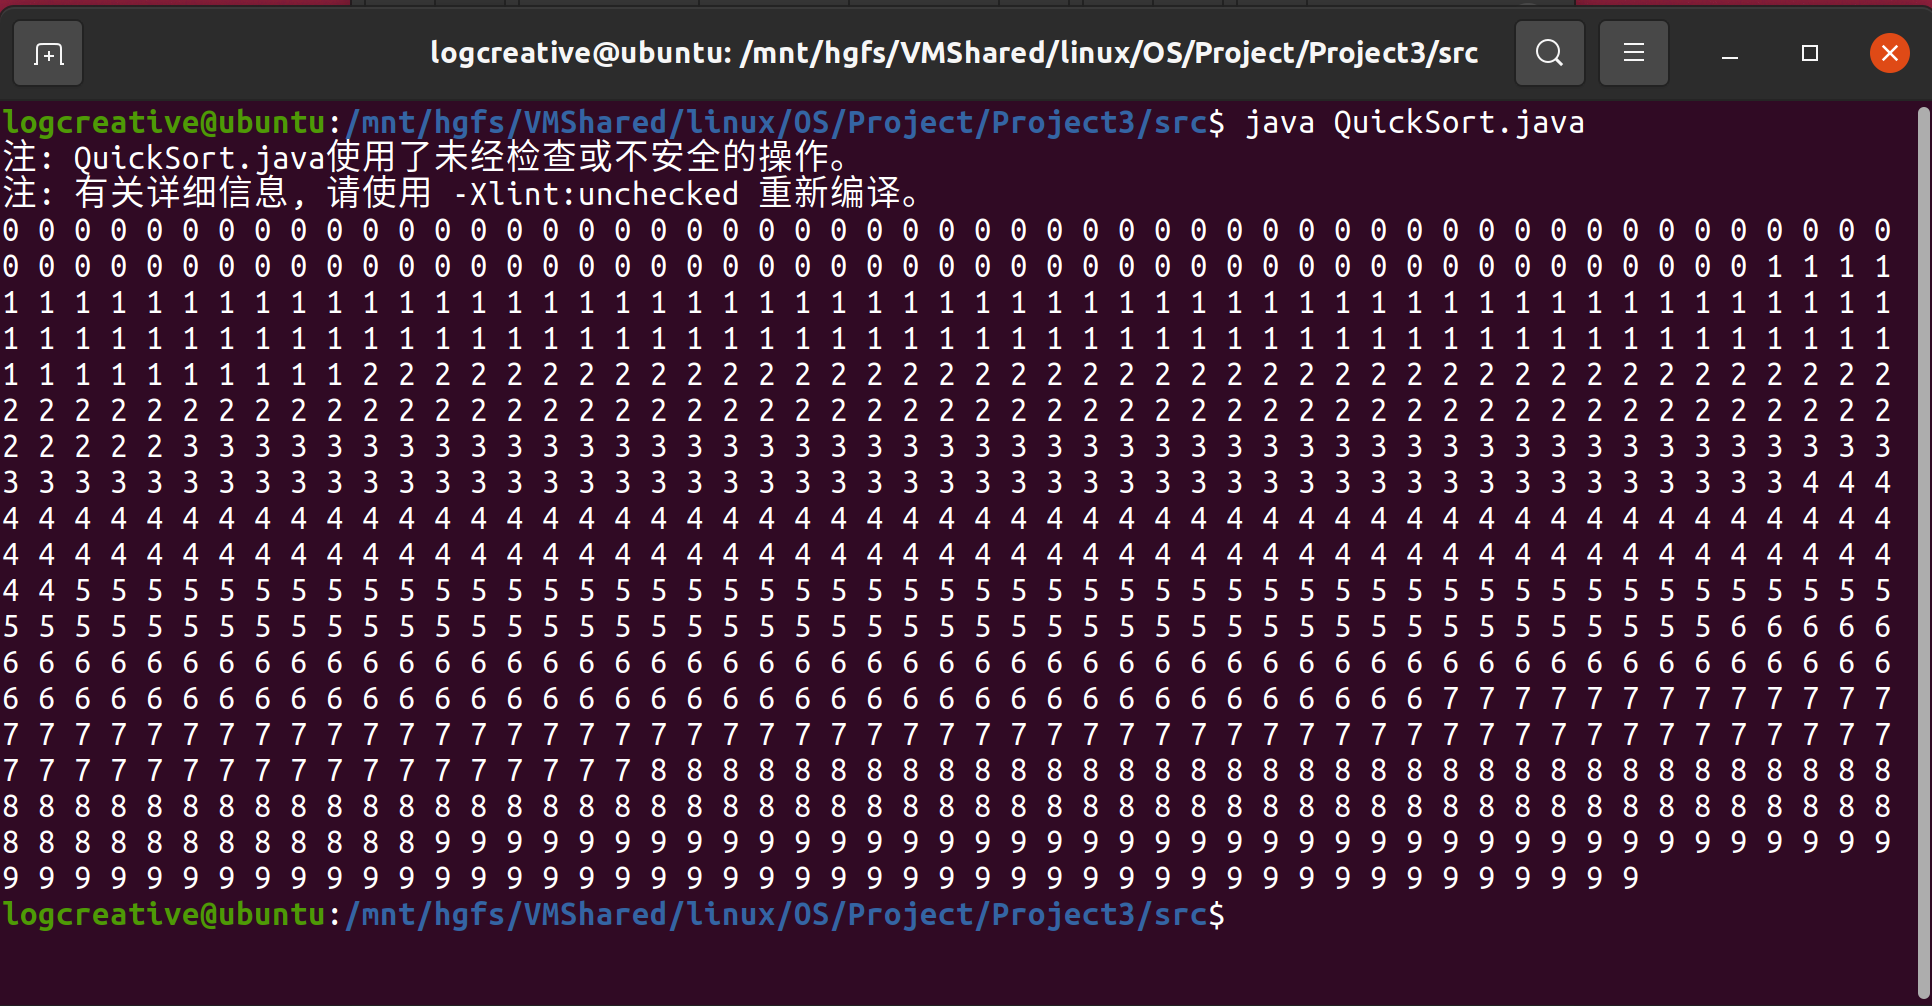
\includegraphics[width=0.9\textwidth]{quicksort.png}

    \code{src/QuickSort.java}{java}

    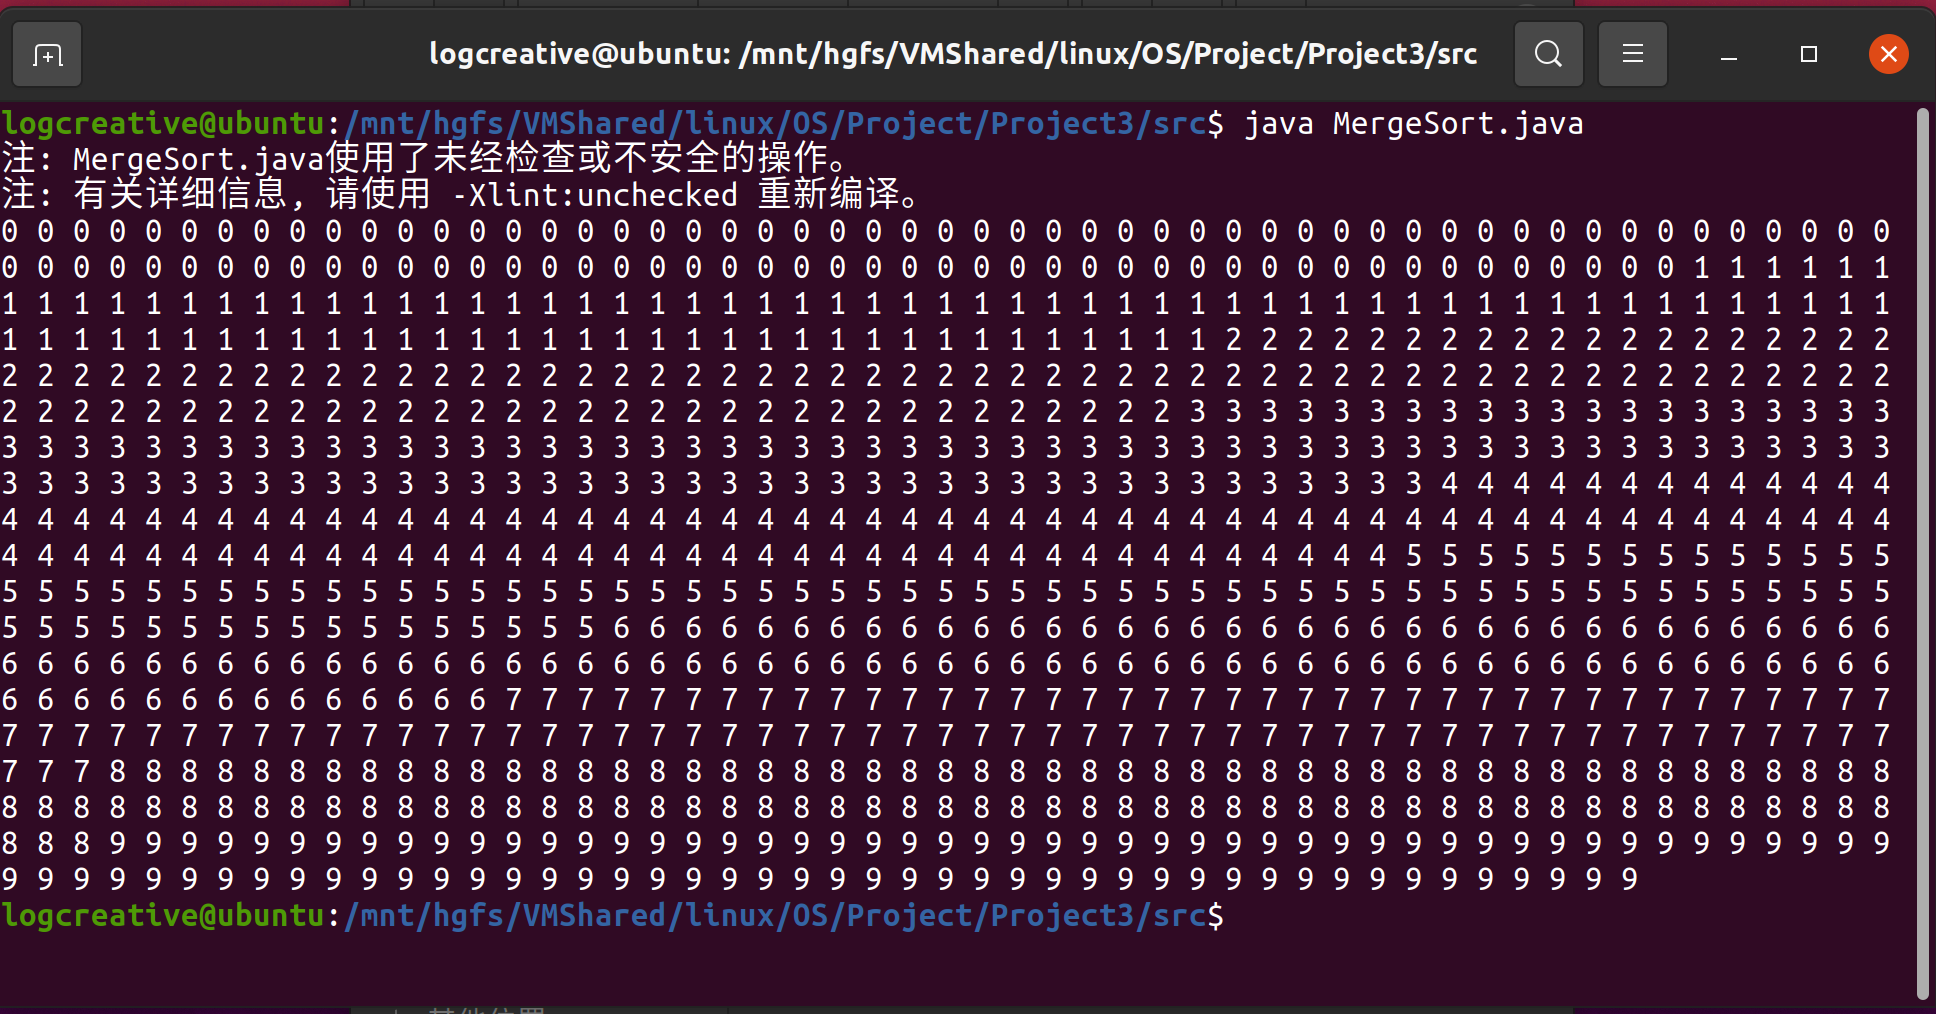
\includegraphics[width=0.9\textwidth]{mergesort.png}

    \code{src/MergeSort.java}{java}

\end{problems}

\end{document}
